% !TEX root=/home/tavant/these/manuscript/src/manuscript.tex

\section{Canonical simulation results}
  \label{sec-canonical}
  
  The {\it canonical} case is the reference case that will be extensively described and commented.
  It will be used then to analyse and quantify the effects of the two aspect of the dielectric walls:
  \begin{itemize}
    \item the dielectric layer on the plasma potential, analysed in  % \cref{sec-dielectric_layer}
    \item the electron emission, analysed in %\cref{sec-see}
  \end{itemize}
  
  
  \Cref{fig-profiles} shows the radial profiles of the electron and ions densities averaged azimuthally.
  We can see the sheath close to the wall where the electron density fall rapidly compare to the ions.
  
  
  \begin{figure}[hbtp]
    \centering
    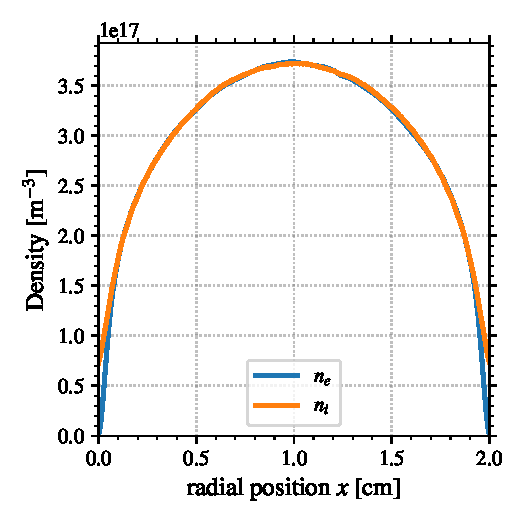
\includegraphics[width=\defaultwidth]{density_profile.pdf}
    \caption{Radial profile of the ion and electron densities at steady state.}
    \label{fig-profiles}
  \end{figure}